\section{Marco teórico}
\subsection{Aprendizaje automático}
%- explicación resumida tipos de aprendizaje (supervisado, no supervisado, semisupervisado)
 Dentro de las diferentes ramas de la inteligencia artificial, los algoritmos utilizados se pueden clasificar en tres grandes ramas según la forma en que son entrenados: algoritmos de aprendizaje supervisado, algoritmos de aprendizaje semi-supervisado y algoritmos de aprendizaje no supervisado. Los primeros son los que se utilizan cuando para el conjunto de entrenamiento \(X\) se tiene un conjunto de etiquetas \(y\) con las que se relacionan unívocamente, y de esta manera, los algoritmos encuadrados dentro de esta rama se encargan de estimar una función que mapee los datos del conjunto \(X\) al conjunto \(y\), con el fin de  luego poder realizar inferencias a partir de sólo nuevos casos de entrada. Los algoritmos de aprendizaje no supervisado se utilizan en situaciones en las que se tiene un conjunto de datos de entrada \(X\) pero no se tiene un conjunto de etiquetas asignadas a estos datos, estos algoritmos se emplean para realizar sobre los datos tareas tales como agrupamientos, detección de anomalías, reducción de dimensionalidad, entre otras. Por último, la rama del aprendizaje semi-supervisado entra en juego para aquellos casos en los que se tiene un pequeño conjunto de datos etiquetado, y un gran conjunto de datos no etiquetados.
 
%- explicación profunda aprendizaje supervisado, ejemplos otros tipos de problemas
 En este trabajo se contará tanto con un conjunto de entrenamiento que serán bases de datos de imágenes como con sus pertenecientes etiquetas, por lo que se intentará mapear mediante algún algoritmo (en este caso técnicas de aprendizaje profundo) cada imagen con sus etiquetas: aprendizaje supervisado.
 
 Dentro de esta rama existen otros algoritmos que pueden servir para este problema o para otros problemas de dominio diferente como son los árboles de decisión, regresiones lineales o logísticas, ensembles, etc.
 
\subsection{Representación de una neurona}
%- explicación neurona
 En este trabajo, como bien se explicó anteriormente, se abordará la solución mediante técnicas de aprendizaje profundo, por lo que a continuación se dara lugar a las explicaciones pertinentes relacionadas a este tipo de técnica.
 Para empezar es necesario comentar que el término "profundo" recae en la profundidad de las redes neuronales que se utilizan en esta técnica. Estas redes pueden estar compuestas hasta por millones de neuronas interconectadas entre si; neuronas que se representan como se observa en la imagen \ref{fig:representacion_neurona} en donde se muestra un ejemplo de una neurona con \(n\) entradas, conformada por: 
 \begin{itemize}
 	\item Entradas: conjunto de datos de entrada \(x_1\)..\(x_n\)
 	\item Pesos: conjunto de pesos \(w_1\)..\(w_n\) correspondientes a cada entrada
 	\item Función de agregación: función que agrega la multiplicación pesada entre cada entrada \(x\) y su correspondiente peso \(w\).
	\item Función de activación: función no lineal responsable de mapear el resultado de la función de agregación en salidas (según que tipo de función los resultados son valores entre [0, 1]o [-1, 1]).
	\item Salida: resultado de la función de activación.
 \end{itemize}
 
 
\begin{figure}
\centering
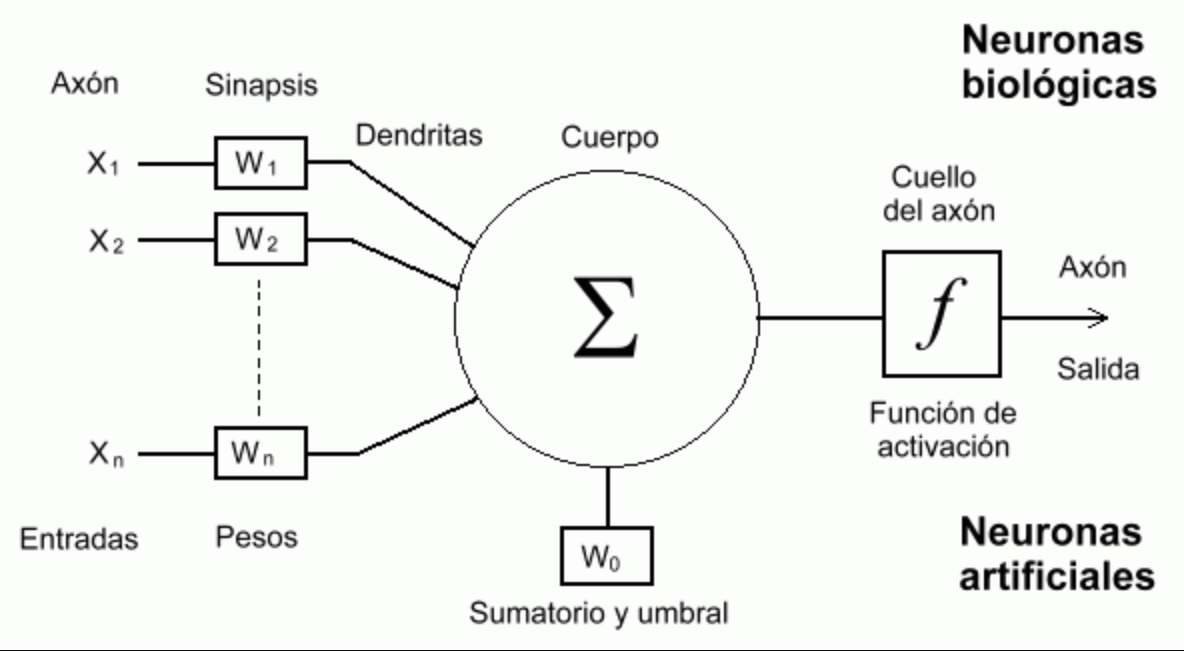
\includegraphics[width=0.7\linewidth]{images/representacion_neurona}
\caption[Representación de una neurona]{Representación de una neurona}
\label{fig:representacion_neurona}
\end{figure}

De esta manera, se puede obtener la salida de la neurona \(Y\), a partir de aplicar la función de activación \(\sigma\) a la suma entre el sesgo \(b\) y la multiplicación matricial del conjunto de entrenamiento \(X\) y los pesos \(W\).

\begin{equation}
Y=\sigma\left(W^{T} X^{(i)}+b\right)
\end{equation}


\subsection{Red Neuronal}

%- explicación redes neuronales profundas
 Una red neuronal, como su nombre lo enuncia, es una consecución de capas de \(N\) neuronas en cada una, conectadas entre sí como se puede ver en el ejemplo de la figura \ref{fig:redneuronal}. Es necesario que se cuente con capas de entrada, capas ocultas y capas de salida; para la figura \ref{fig:redneuronal} se tiene una capa de entrada, dos capas ocultas y una capa de salida. 
 El fin de las redes neuronales es aprender representaciones del contenido de la información en relación a las salidas esperadas para luego poder hacer inferencias en nuevo contenido, a modo de ejemplo, si se tienen imágenes de perros y gatos, y el fin es detectar si se trata de un perro o un gato la red posiblemente no aprenda las mismas representaciones que si el fin de la misma es detectar presencia o ausencia de animales.
 
 
 
 \begin{figure}
 	\centering
 	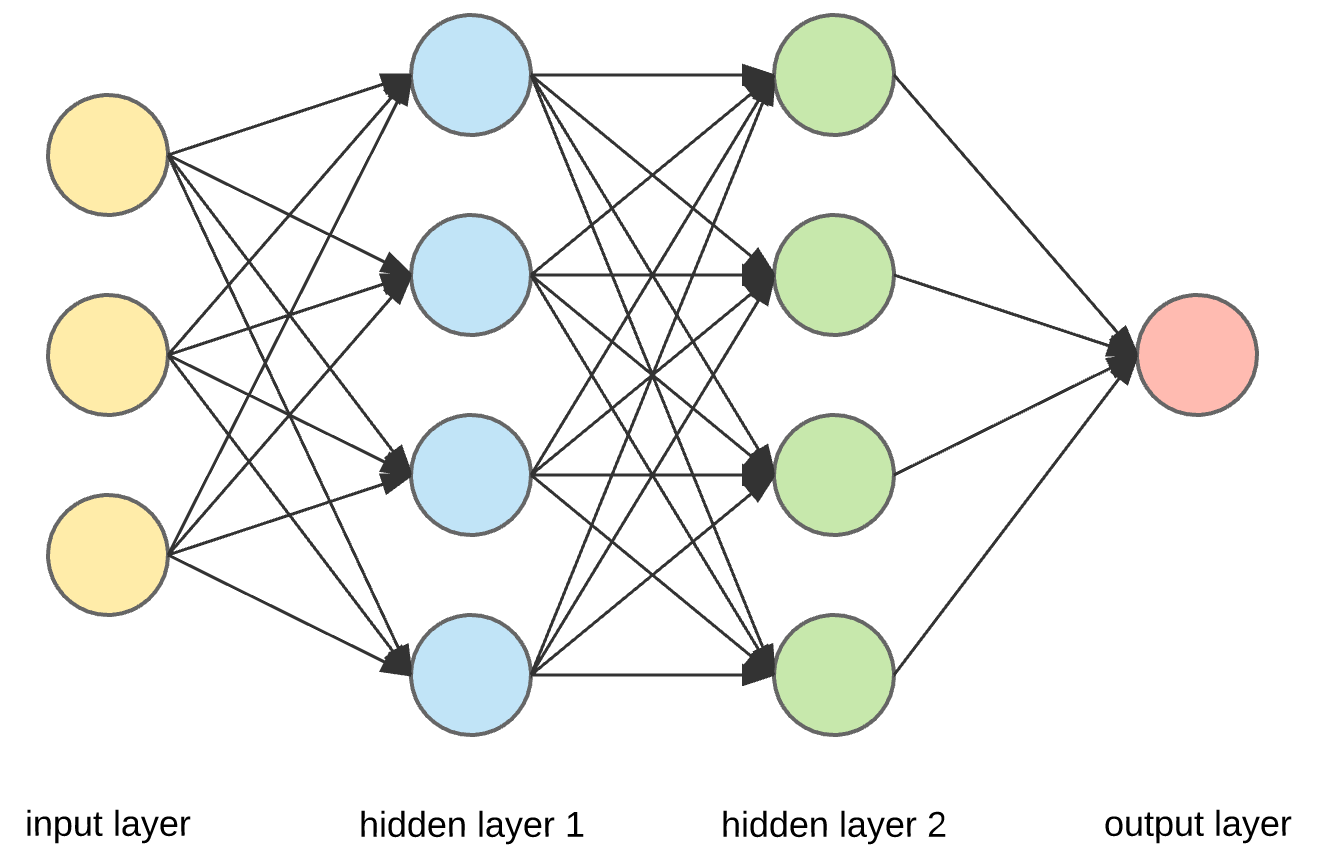
\includegraphics[width=0.7\linewidth]{images/red_neuronal}
 	\caption[Ejemplo red neuronal]{Perceptrón Multi Capa}
 	\label{fig:redneuronal}
 \end{figure}

 Para explicar el funcionamiento de las redes neuronales es necesario también introducir algunos conceptos como son la propagación hacia adelante y hacia atrás, función de pérdida y optimización. Durante la fase de entrenamiento, los pasos que se siguen son:
 \begin{enumerate}
 	\item Propagación hacia adelante
 	\item Evaluación de función de pérdida
 	\item Propagación hacia atrás
 \end{enumerate}
 La propagación hacia adelante es la actividad en la que se le brindan los datos a la capa de entrada de la red para que se evalúen todas las capas en esa dirección aplicando \ref{formula:forward_prop} en cada capa tomando como entrada la capa inmediata anterior. De esta manera, se obtiene como salida de la red sus predicciones. Luego, a partir de estos resultados es posible medir la función de pérdida, a partir de la cual se realiza la propagación hacia atrás del error.
  
 \begin{equation}\label{formula:forward_prop}
 z=W^{\wedge} T x+b
 \end{equation}
 


- explicacion funcionamiento:
	- forward prop 
	- back prop
	- regularizers:
		- dropout
		- batch norm
	- optimizers
	- metrics
	- loss functions
	
\subsection{Red Neuronal Convolucional}
- explicación razón de convoluciones
- partes:
	- Convolución
	- stride
	- pooling layers
- ejemplo simple

\subsection{Redes preentrenadas} 
- Transfer Learning
- Arquitecturas de las redes y datasets ejemplos

\subsection{Representación del conocimiento}
- Ejemplos activaciones